\documentclass[11pt, oneside]{article}
\usepackage[margin=1in]{geometry}
\geometry{letterpaper}
\usepackage{amssymb}
\usepackage[fleqn]{amsmath}
\usepackage[sharp]{easylist}
\usepackage{relsize}
\usepackage{graphicx}

\pagenumbering{gobble}              % No page numbering
\setlength{\parindent}{0em}         % No paragraph indenting
\setlength{\parskip}{0.5em}         % Paragraph spacing

\newcommand*{\begineasylist}{\begin{easylist}[itemize]\ListProperties(Style*=$\bullet$\quad, Style2*=\tiny$\blacksquare$\quad, Style3*=$\circ$\quad, Style4*=$\diamond$\quad, FinalSpace=1em, Space=0em, Space*=0em)}

\newcommand*{\begineasylistnumbered}{\begin{easylist}[enumerate]\ListProperties(Numbers=a, Space=0em, Space*=0em)}

\begin{document}

\section*{CS 247 Midterm Review}

\subsection*{ADT Design}
\begineasylist

# Bullet point here



\end{easylist}
\subsection*{Documentation}
\begineasylist




\end{easylist}
\subsection*{Exceptions}
\begineasylist




\end{easylist}
\subsection*{RAII Idiom}
\begineasylist




\end{easylist}
\newpage
\subsection*{UML}
\begineasylist

# \textbf{Unified Modelling Langauge}

# Class diagrams
## Attributes
### \texttt{[visibility] name: [type] [multiplicity] = [default value] \{property\}}
## Operations
### \texttt{[visibility] name (parameter list) : [return type] \{property\}}
### + public; - private; \# protected; \underline{static}; \emph{pure virtual}
### \texttt{property} = read-only (aka. const), query (aka. accessor), abstract, etc.

# Associations: physical or conceptual links between classes
## Classes being associated may have \underline{role names}
## Navigability: direction of association; e.g. A \emph{has} B

# Multiplicity (of attributes or associations)
## $a$: exactly $a$
## $m..n$: between $m$ and $n$
## $*$: many (at least zero)

# Aggregate: a \underline{collection} of \underline{members}
## Collection has many members
## Member can belong to many collections, or exist independently
## Collection is \underline{not responsible} for its members

# Composition: a stricter collection of members
## Member cannot exist without its collection
## Member belongs to exactly one collection
## Collection is \underline{responsible} for its members

# Generalization = inheritance

# Sequence diagrams: describe how information is passed between objects (e.g. via function calls), throughout execution of a program


\end{easylist}
\newpage
\subsection*{Design Patterns}
\begineasylist

# \textbf{Inheritance}
## Parent class's methods are inherited by child classes
### Classes' methods share the same implementation structure
### Only differences are the data values
## Downside: not all subclasses may want to inherit parent behaviour
## Downside: code duplication

# \textbf{Strategy pattern}
## Allows the implementation of an algorithm/method to be changed at runtime \\(\underline{encapsulation of algorithm})
## Allows the algorithm \underline{vary independently from clients} that use it
## e.g. data structure holds an instance of base Strategy class, calls the algorithm/method (which is \emph{pure virtual} in base class)
### Concrete methods with differing behaviour are implemented in Strategy subclasses
### Strategy can be changed (to other subclasses) at runtime, changing the method's behaviour

\begin{figure}[!ht]
    \centering
    \includegraphics[width=0.8\textwidth]{res/strategy.png}
\end{figure}

# \textbf{Template pattern}
## \textbf{Template method} is a method in a base class that defines code structure but leaves \underline{holes} to be defined by subclasses
## Holes are operations defined as \emph{pure virtual} in the base class, but have varying implementations in subclasses

\begin{figure}[!ht]
    \centering
    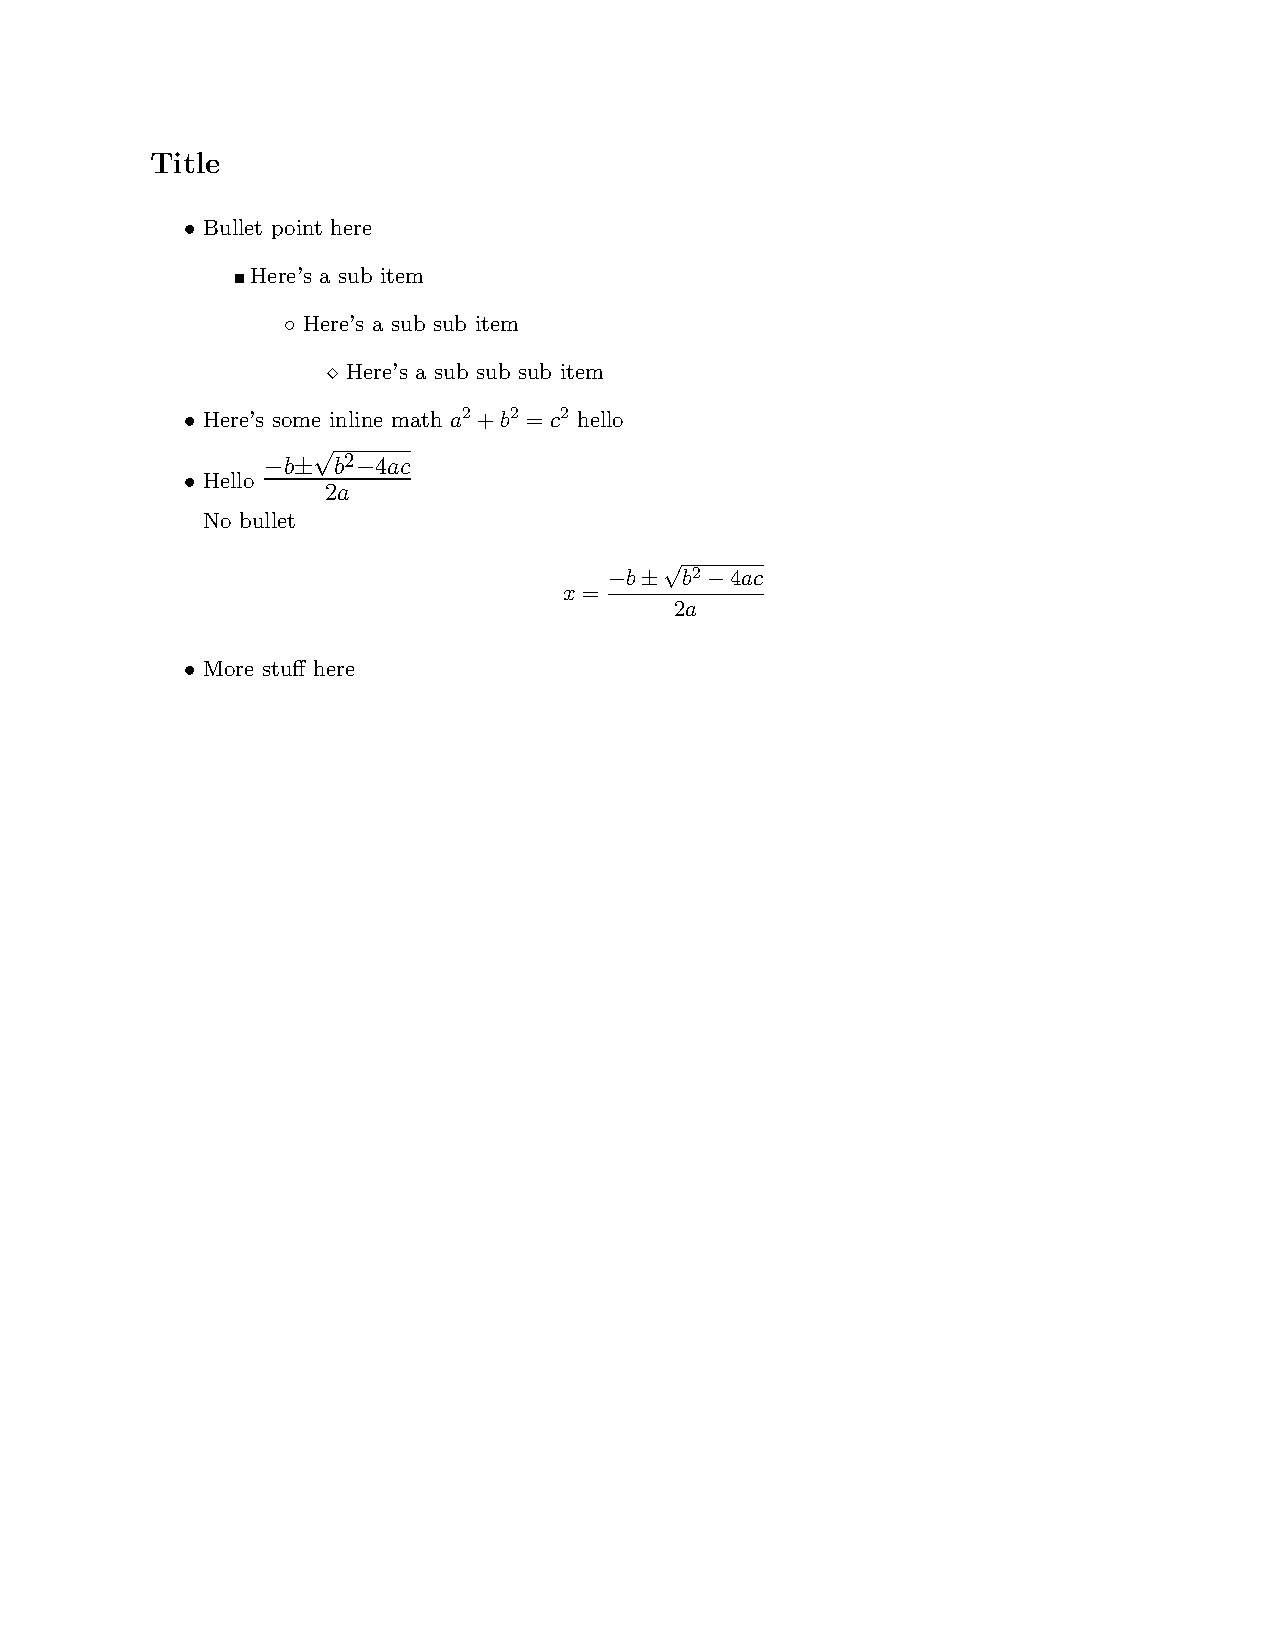
\includegraphics[width=0.6\textwidth]{res/template.png}
\end{figure}

\newpage

# \textbf{Adapter pattern}
## Adapter \underline{maps one interface to another}
## e.g. interfaces of an existing module does not match with a new module
## e.g. wrapping an existing data structure interface to create a new data structure

\begin{figure}[!ht]
    \centering
    \includegraphics[width=0.7\textwidth]{res/adapter.png}
\end{figure}

# \textbf{Facade pattern}
## Simplies and unifies classes and interfaces in a subsystem into only a high-level interface and hides individual interfaces within the subsystem
## Subsystem components and interfaces can be changed without affecting client

\begin{figure}[!ht]
    \centering
    \includegraphics[width=0.7\textwidth]{res/facade.png}
\end{figure}

# \textbf{Singleton pattern}
## Ensures \underline{only one instance} of a class can exist
## Private constructor; only instantiated through static \texttt{getInstance()} method

\newpage
# \textbf{Observer pattern}
## Subject $\rightarrow$ (one-to-many) Observers
## Subject can notify all subscribed observers to update
## Observers can subscribe/unsubscribe at runtime
## \textbf{Push model}: subject pushes state information to observers through \texttt{notify(State)}
## \textbf{Pull model}: subject notifies observers, who request information via subject's accessors
## \textbf{Loose coupling}: subjects and observers only know about each other's interfaces, not the concrete classes that implement them

\begin{figure}[!ht]
    \centering
    \includegraphics[width=0.6\textwidth]{res/observer.png}
\end{figure}

# \textbf{MVC pattern}
## UI code is abstracted into the \textbf{view}
### Composite pattern: all view elements use the same base class (uniform interfaec)

## \textbf{Controller} translates user input (from the view) into operations on the model
### Strategy pattern: controller provides the view with a strategy; controller behaviour can be changed by swapping for a different strategy

## \textbf{Model} holds data, state, and application logic
### Observer pattern: model = subject; views = observers; model sends out notification on state change, triggering views to update accordingly

\end{easylist}
\newpage
\subsection*{OOP Principles}
\begineasylist

# \textbf{Open Closed Principle}
## Modules should be \underline{open} for extension but \underline{closed} for modification
## ``Program to an interface, not an implementation''
## e.g. provide an abstract base class (may have default implementation) that can be extended by the client

# \textbf{Composition Over Inheritance}
## Composition = include base class in new subclass as a complex attribute
### i.e. ``has-a'' instead of ``is-a''
## Choose inheritance when subtyping/polymorphism, or when base class's entire interface is required
## Choose composition for non-overriding reuse because the base component can be changed at runtime
## Composite object can \underline{delegate} operations to component objects

# \textbf{Single-Responsibility Principle}
## Each changeable design decision should be encapsulated in a module

# \textbf{Liskov Substitutability Principle}
## A derived class must be substitutable for its base class
### Must accept the same messages (method signatures match the base class)
### Derived methods must \underline{require no more} (weaker or same preconditions) and \underline{promise no less} (stronger or same postconditions) than base class methods
### Derived class must preserve properties of base class (e.g. invariant, performance)

# \textbf{Law of Demeter}
## An object should only ``talk to its neighbours''
## A method \texttt{C::m()} can only call methods of:
### C
### C's members
### m's parameters
### Any object constructed by A's methods
## Prevents calling a chain of methods to perform an operation/retrieve information


\end{easylist}

\end{document}